\clearpage{\pagestyle{empty}\cleardoublepage}
\chapter{Analisi qualitativa delle immagini} 
\label{appendiceWSS} 

Anche dalla semplice osservazione delle immagini è possibile notare i cambiamenti apportati dall'algoritmo.

\begin{figure}
 \centering
 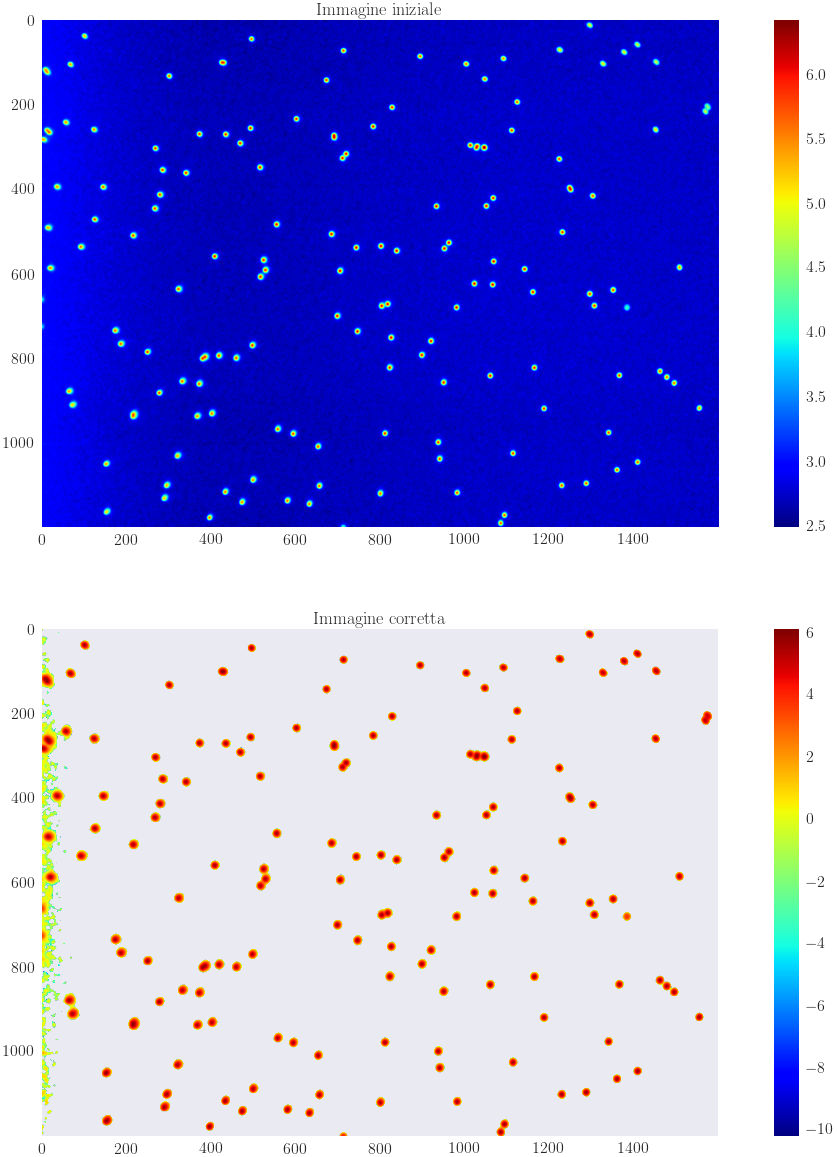
\includegraphics[scale=.40]{img/CAP4lg1.png}
 \caption{\small{Evoluzione dell'immagine di calibrazione con sfere a fluorescenza omogenea: in alto è raffigurata l'immagine acquisita col microscopio a fluorescenza e in basso quella risultante dopo aver corretto la disomogeneità di illuminazione. Le immagini, rappresentate nella color map ``jet'' riportata a fianco, sono i logaritmi delle corrispettive immagini originali, a cui è stato applicato ulteriormente il filtro gaussiano.}}
 \label{fig:lg1}
\end{figure}

In \figurename~\ref{fig:lg1} è possibile notare la sostanziale correzione del difetto della luminosità disomogenea: le sferette aventi stessa intensità, originariamente percepite con differente luminosità, vengono rappresentate dopo la correzione con una medesima tonalità di colore, mostrando così in modo più fedele la realtà del campione.

\begin{figure}
 \centering
 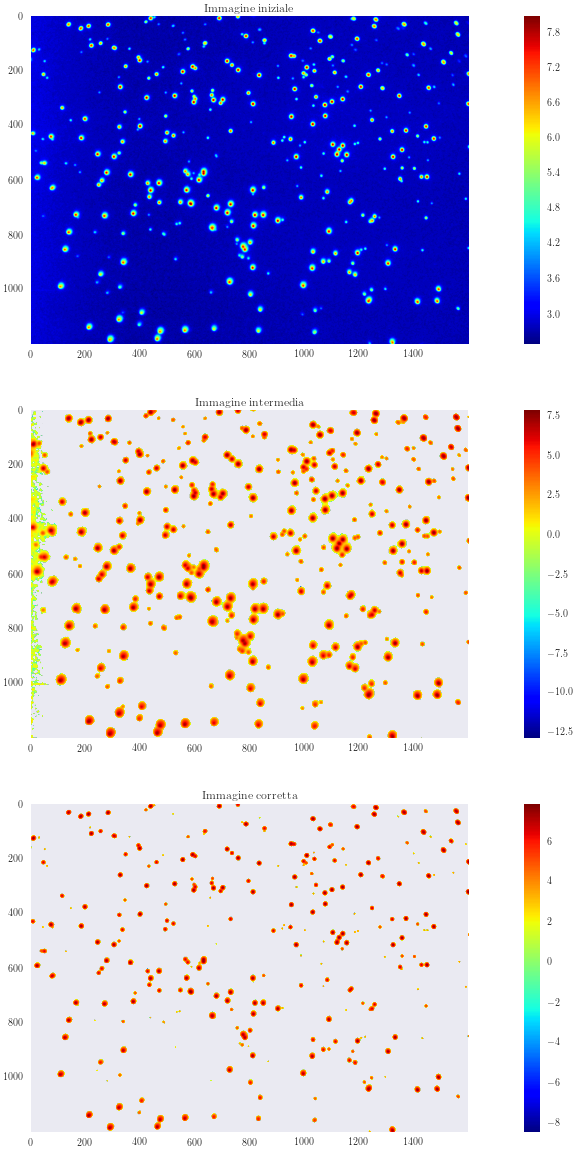
\includegraphics[scale=.50]{img/CAP4lg2.png}
 \caption{\small{Evoluzione dell'immagine di calibrazione con sfere aventi differenti intensità di fluorescenza: in alto è raffigurata l'immagine acquisita col microscopio a fluorescenza, al centro quella risultante dopo aver corretto la disomogeneità di illuminazione e in basso l'immagine privata del parametro costante di background. Le immagini, rappresentate nella color map ``jet'' riportata a fianco, sono i logaritmi delle corrispettive immagini originali, a cui è stato applicato ulteriormente il filtro gaussiano.}}
 \label{fig:lg2}
\end{figure}

Nell'evoluzione dell'immagine di calibrazione delle sferette aventi cinque intensità differenti (\figurename~\ref{fig:lg2}) è possibile notare, oltre alla correzione della disomogeneità spaziale, anche la rimozione della fluorescenza residua di sfondo.

\begin{figure}
 \centering
 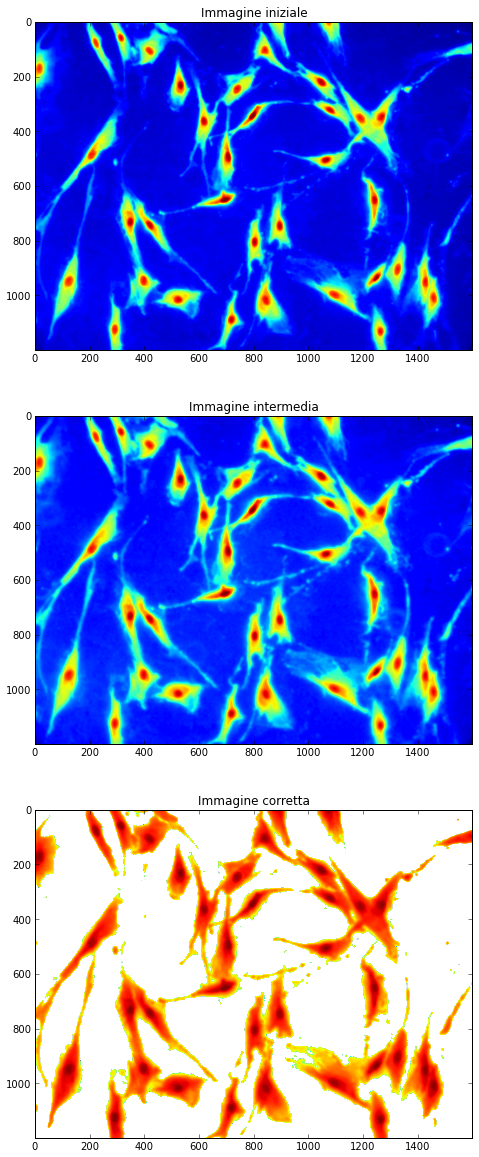
\includegraphics[scale=.50]{img/CAP4lg3.png}
 \caption{\small{Evoluzione dell'immagine delle cellule di fibroblasti: in alto è raffigurata l'immagine acquisita col microscopio a fluorescenza, al centro quella privata dei parametri costanti di background e in basso l'immagine risultante dopo aver corretto la disomogeneità di illuminazione. Le immagini, rappresentate nella color map ``jet'' riportata a fianco, sono i logaritmi delle corrispettive immagini originali, a cui è stato applicato ulteriormente il filtro gaussiano.}}
 \label{fig:lg3}
\end{figure}

\begin{figure}
 \centering
 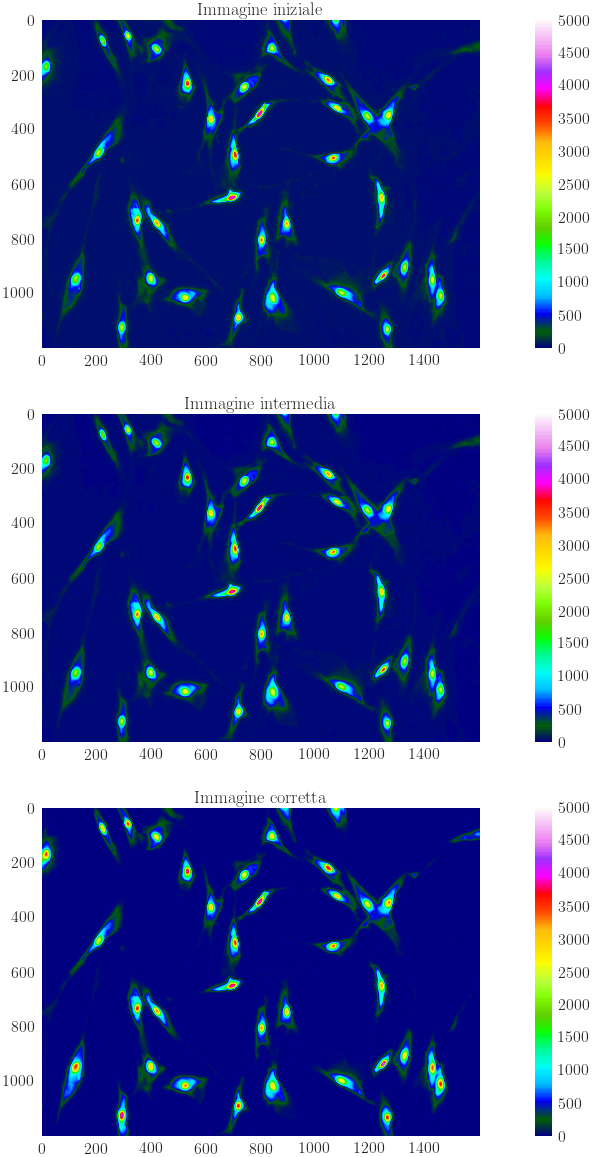
\includegraphics[scale=.50]{img/CAP4cmap.png}
 \caption{\small{Evoluzione dell'immagine delle cellule di fibroblasti: in alto è raffigurata l'immagine acquisita col microscopio a fluorescenza, al centro quella privata dei parametri costanti di background e in basso l'immagine risultante dopo aver corretto la disomogeneità di illuminazione. Le immagini, rappresentate nella color map ``gist\_ncar'' riportata a fianco, sono le corrispettive immagini originali a cui è stato applicato il filtro gaussiano.}}
 \label{fig:cmap}
\end{figure}

Per quanto riguarda l'immagine delle cellule di fibroblasti, vero target dell'algoritmo di correzione, il cambiamento risulta davvero ben evidente: il difetto dei bordi è fortemente attenuato, infatti i nuclei più a margine riacquistano una colorazione molto più intensa e confrontabile con quella dei nuclei centrali, ed inoltre il background viene pressoché portato a zero, il tutto mantenendo ben definiti i confini delle varie cellule.
Le varie fasi correttive dell'immagine sono rappresentate sia in (\figurename~\ref{fig:lg3}) che in (\figurename~\ref{fig:cmap}).